\begin{frame}{Count models}
  \begin{columns}
    \begin{column}{0.65\textwidth}
      \begin{itemize}
        \item Used when modeling counts of items
        \item Predicts probability of integer outcomes
        \item ...therefore, is a discrete choice model
      \end{itemize}
    \end{column}~%
    \begin{column}{0.34\textwidth}
      
\includegraphics[width=\textwidth]{img/countvoncount.png}\\
      {\tiny\hfill\copyright~Sesame Workshop}
    \end{column}
  \end{columns}
\end{frame}

\begin{frame}{Count models: why not linear regression?}
  \only<1-2,4-5>{\centering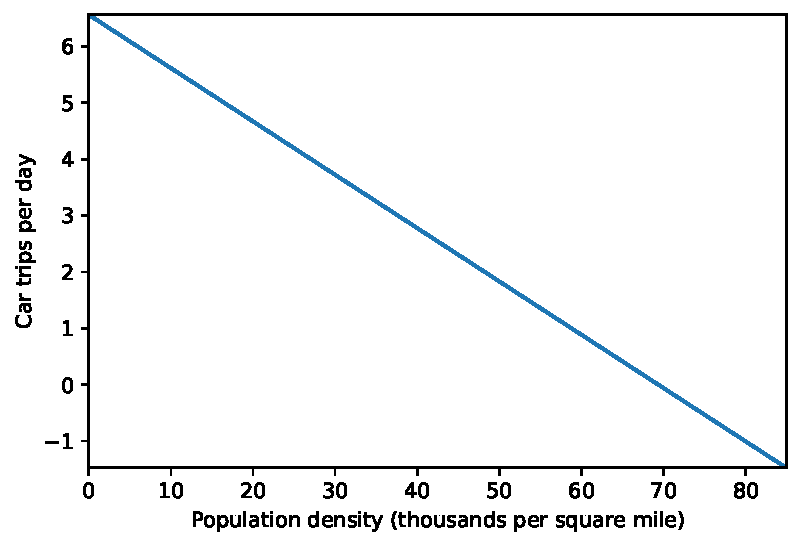
\includegraphics[width=0.6\textwidth]{fig/lincarown.pdf}}
  \only<3>{\centering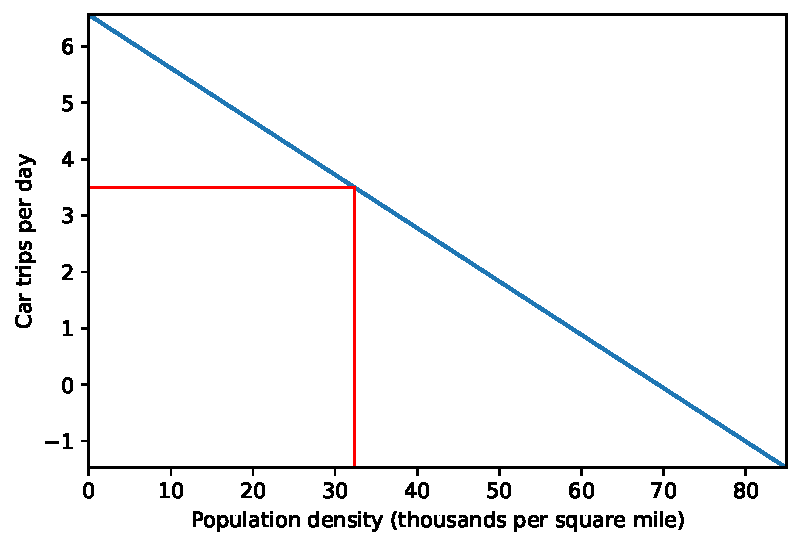
\includegraphics[width=0.6\textwidth]{fig/lincarown_nonint.pdf}}
  \only<6>{\centering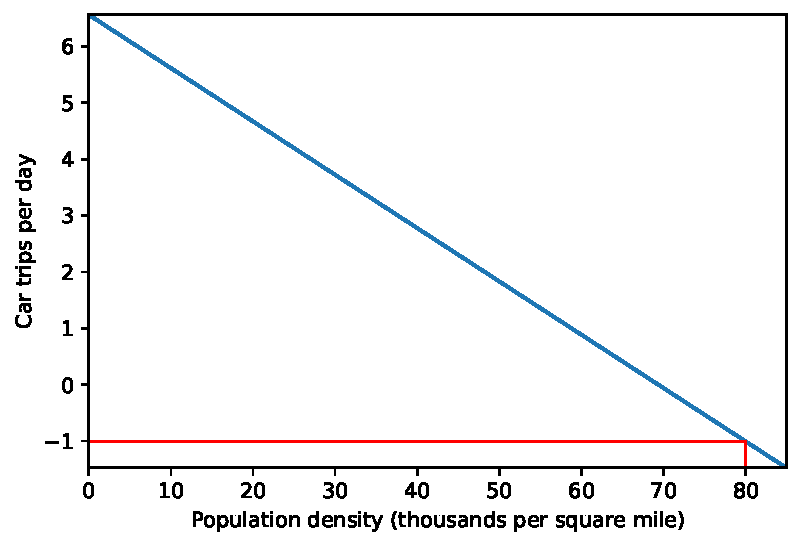
\includegraphics[width=0.6\textwidth]{fig/lincarown_neg.pdf}}
  ~\\
  \only<2-3>{What is the predicted vehicle ownership in a neighborhood with 32,000 people per square mile?}
  \only<5-6>{What is the predicted car ownership in a neighborhood with 71,000 people per square mile?}
  ~\\
  \tiny\citenhts
\end{frame}

\begin{frame}{Poisson regression}
  \begin{itemize}
    \item Poisson regression solves these problems by modeling counts using a \emph{Poisson distribution}
    \item Poisson distribution is discrete, defined only for nonnegative integers
    \item The mean of the distribution is modeled as $\mu = e^{\alpha + \beta_1 x_1 + \cdots + \beta_n x_n}$
    \item This determines the probabilities for all possible counts
    \item Thus, Poisson is a \emph{multiplicative} model
    \item $e^\beta$ is the \emph{incidence rate ratio}, ratio of expected counts when variable increase by one
  \end{itemize}
\end{frame}

\begin{frame}{Poisson regression: example}
  \centering\begin{tabular}{lrrrr}
  \toprule
  {} &  Coefficient &  Incidence rate ratio &  Std. err. &  p-value \\
  \midrule
  Constant    &     1.887 &              &   0.001 &      0.0 \\
  Population density &    -0.017 &              0.983 &   0.0 &      0.0 \\
  (thousands per square mile) & & & & \\
  \bottomrule
  \end{tabular}\\
  \tiny\citenhts
\end{frame}

\begin{frame}[label=pois]{Poisson regression: example}
  \centering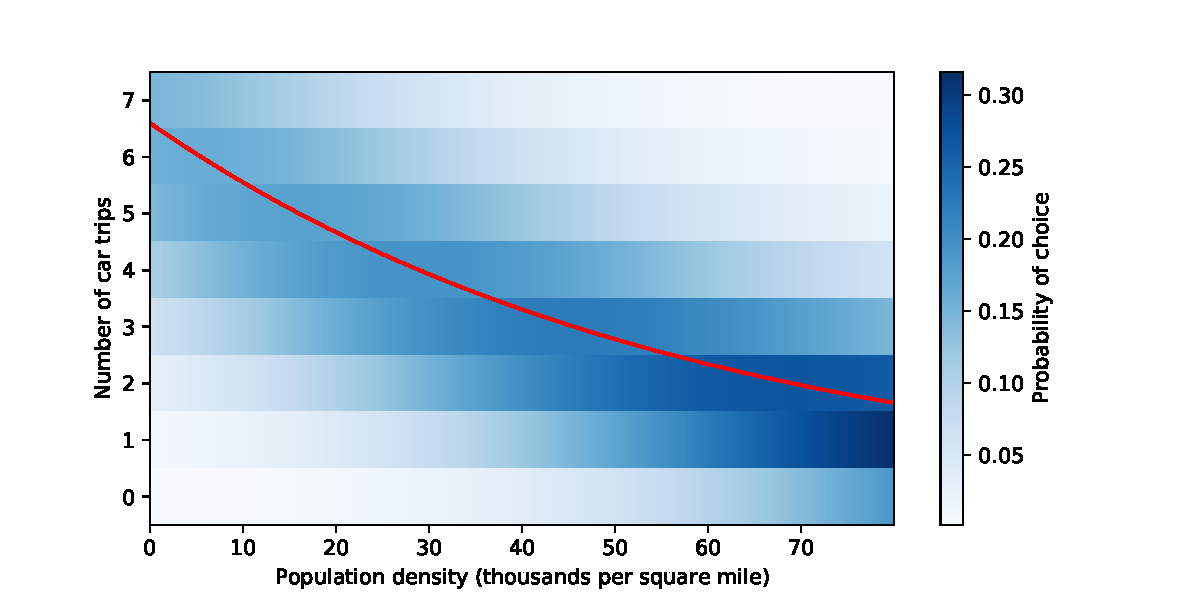
\includegraphics[width=0.75\textwidth]{fig/poisson.pdf}\\
  \tiny\citenhts
\end{frame}

\begin{frame}{Negative binomial regression}
  \begin{itemize}
    \item Poisson regressions assumes that the standard deviation of the error term is the same as the mean
    \item This is a result of the derivation of the Poisson distribution from the binomial distribution
    \item Assumes that the model predicts perfectly
    \pause\item ...which is never true
  \end{itemize}
\end{frame}

\begin{frame}{Negative binomial regression}
  \begin{itemize}
    \item Negative binomial regression replaces the Poisson distribution with the negative binomial
    \item Adds a parameter $\alpha$ that models the standard deviation of the error term
    \item When $\alpha = 0$ or $\mathrm{ln} \alpha = 1$, equivalent to Poisson
    \item When $\alpha > 0$ or $\mathrm{ln} \alpha > 1$, errors are \emph{overdispersed}
    \item When $\alpha < 0$ or $\mathrm{ln} \alpha < 1$, not consistent with negative binomial assumptions
    \item Basically, negative binomial makes estimates less certain to account for errors in prediction
  \end{itemize}
\end{frame}

\begin{frame}{Negative binomial regression: example}
  \centering\begin{tabular}{lrrrr}
\toprule
{} &  Coefficient &  Incidence rate ratio &  Std. err. &  p-value \\
\midrule
Constant    &     1.893 &              &   0.003 &      0.0 \\
Population density &    -0.019 &              0.981 &   0.0 &      0.0 \\
(thousands per square mile) &&&&\\
$\alpha$    &     \tikzmark{alpha}0.675 &               &   0.004 &      0.0 \\
\bottomrule
\end{tabular}\\
\tiny\citenhts

\pause\begin{tikzpicture}[overlay, remember picture]
  \draw[red] ([xshift=0.75cm]pic cs:alpha) ellipse (1.5cm and 0.5cm);
\end{tikzpicture}
\end{frame}
%
\begin{frame}{Negative binomial regression: example}
  \centering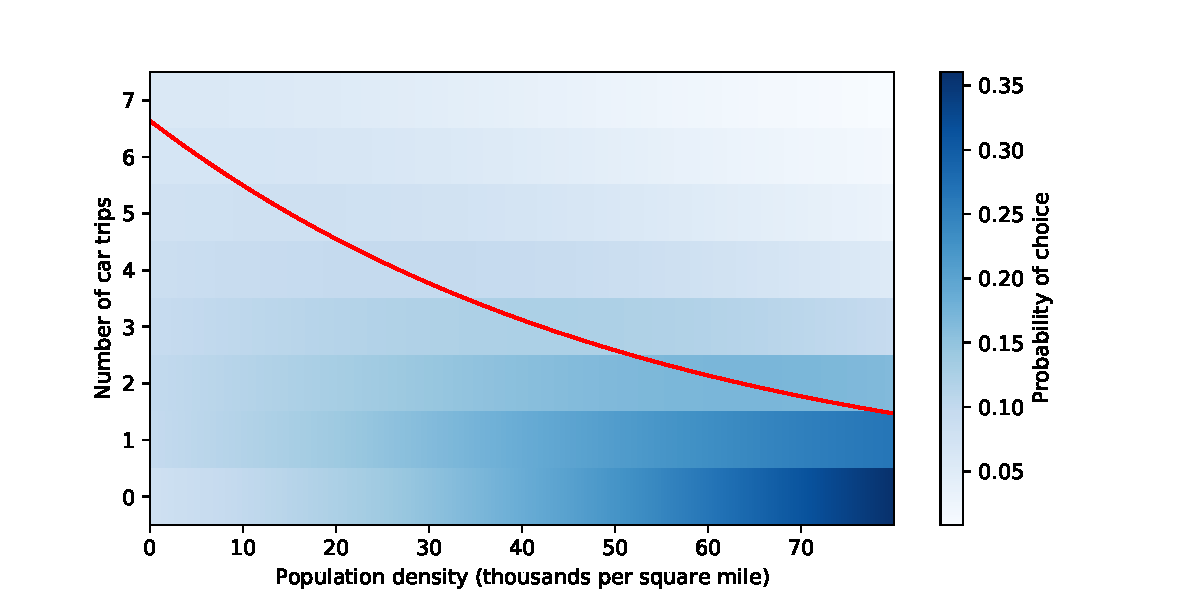
\includegraphics[width=0.75\textwidth]{fig/negbin.pdf}\\
  \tiny\citenhts
\end{frame}
\againframe{pois}

\begin{frame}{Zero-inflated models}
  \begin{itemize}
    \item Sometimes count data have more zeros than expected
    \item One solution is to use \emph{zero-inflated} models
    \item These models hypothesize two reasons for a zero
    \begin{enumerate}
      \item Structural: that observation must always\footnote{almost} be zero (e.g. households without cars)
      \item Chance: no events were observed by chance (e.g. households that decided not to go out by car on the travel day)
    \end{enumerate}
  \end{itemize}
\end{frame}

\begin{frame}{Zero-inflated models}
  \begin{itemize}
    \item Zero-inflated models estimate a binary model for the structural zeros, and a count model for the remaining observations
    \item Models do not have to use the same variables
    \item Zero-inflated Poisson and zero-inflated negative binomial are both available
  \end{itemize}
\end{frame}

\begin{frame}{Zero-inflated models: example}
  \centering\begin{tabular}{lrrrr}
\toprule
{} &  Coefficient &  Incidence rate ratio &  Std. err. &        p-value \\
\midrule
\textbf{Zero-inflation model} \\
Constant    &    -2.234 &   &   0.012&   0.0 \\
No driver in household &     3.220 &             25.025 &   0.037 &   0.0 \\
\midrule
\textbf{Count model} \\
Constant            &     1.99 &              7.283 &   0.003 &   0.0 \\
Population density         &    -0.010 &              0.990 &   0.0 &  0.0 \\
(thousands per square mile) &&&& \\
$\alpha$            &     0.355 &              &   0.003 &   0.0 \\
\bottomrule
\end{tabular}\\
\tiny\citenhts
\end{frame}

\begin{frame}{Zero-inflated models: example}
  \only<1>{\centering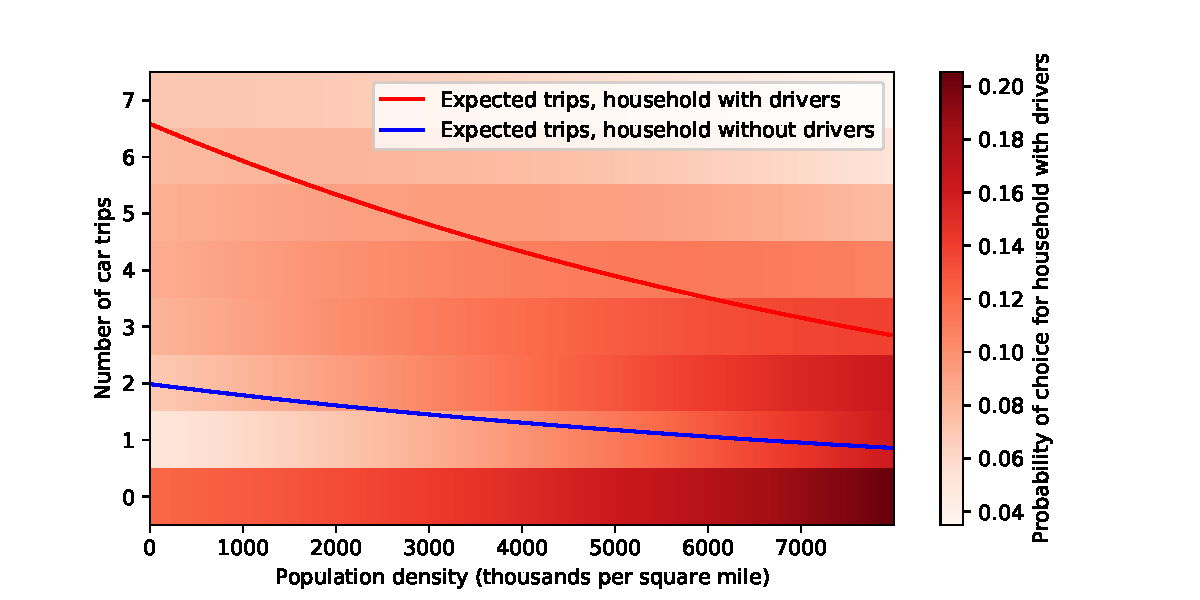
\includegraphics[width=\textwidth]{fig/zinb_driver.pdf}}
  \only<2>{\centering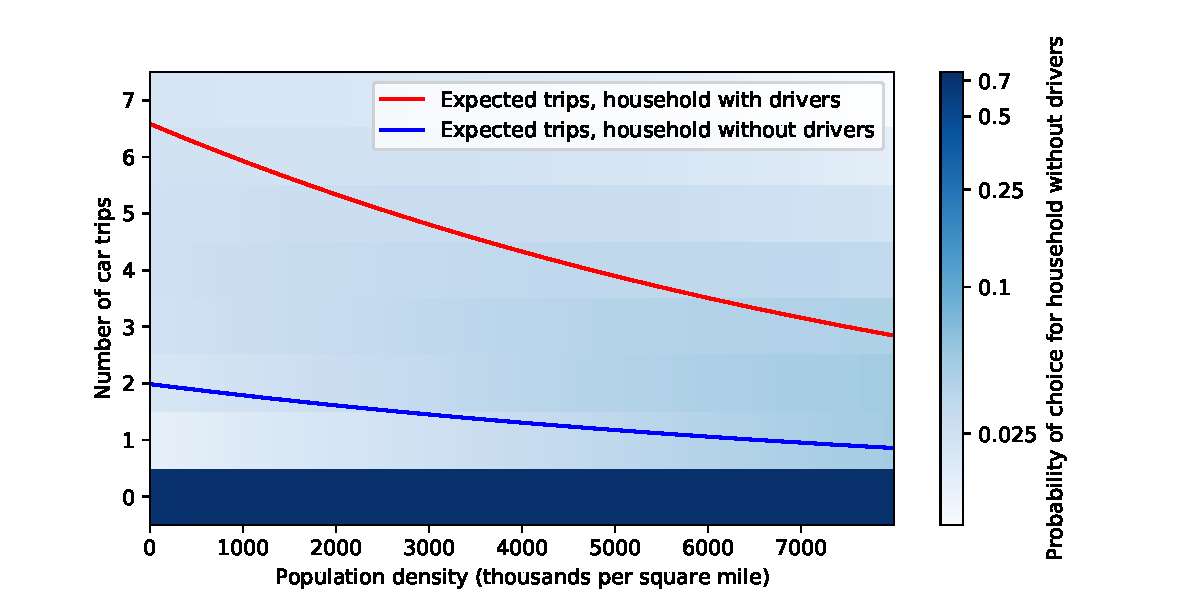
\includegraphics[width=\textwidth]{fig/zinb_nodriver.pdf}}
  \\
  \tiny\citenhts
\end{frame}

\begin{frame}{Zero-inflated $\tau$ models}
  \begin{itemize}
    \item In a zero-inflated $\tau$ (tau) model, there is not a separate set of coefficients for the binary model
    \item Rather, a single coefficient $\tau$ is estimated that scales the coefficients from the count model to predict the structural zeros
    \item Assumes same relative contribution of variables to count and structural zeros
  \end{itemize}
\end{frame}

\begin{frame}{Interpreting count models}
  \begin{itemize}
    \item Much like interpreting linear regression with a logged dependent variable
    \item When incidence rate ratios are presented, they are easy to interpret
    \item Otherwise, positive coefficients mean larger counts, negative means smaller
    \item Zero-inflated models: must account for effects from both count and zero-inflation model
  \end{itemize}
\end{frame}

\begin{frame}{Interpreting count models: example}
  \centering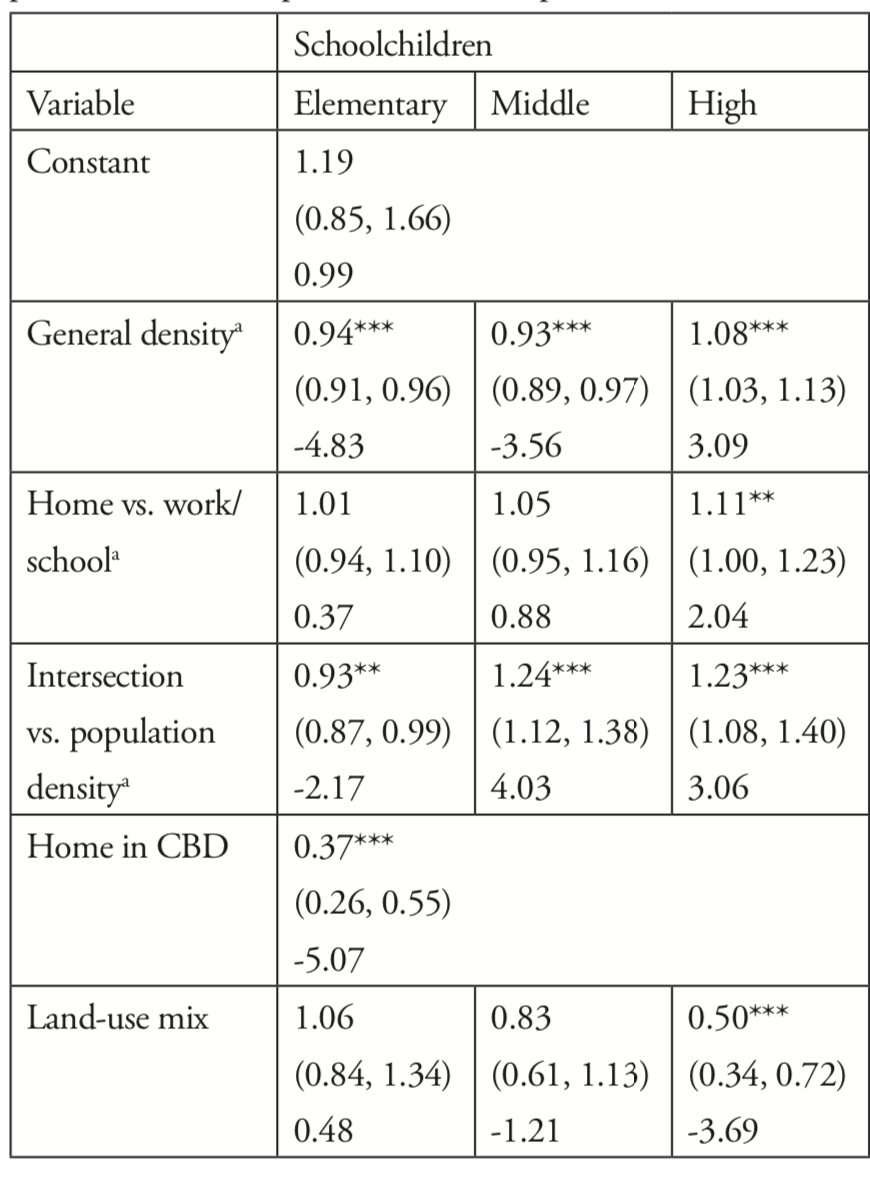
\includegraphics[width=0.35\textwidth]{img/salon_count.png}\\
  {\tiny\textcite{salon_heterogeneity_2019}}
\end{frame}
